% You need .tex/ from http://github.com/scy/dotscy to TeX this file.
\input{presentation.tex}

\title{Git für alle}
\subtitle{Trau dem Hype}
\author[Tim~„Scytale“~Weber]{Tim~„Scytale“~Weber\only<presentation>{\hspace{200em}} <\texttt{scy-talk-git@scytale.name}>}
\institute[oqlt~e.V.]{Organisierte Querdenker für~langfristige Technologiefolgenabschätzung (oqlt~e.V.)}
\date[MRMCD 0x08h]{8. MetaRheinMain ChaosDays, September 2009}
\UseOverviews
\def\HW{{\color{red}$^\star$}}

\begin{document}

\begin{frame}\maketitle\end{frame}

\begin{abstract}
Das Versionskontrollsystem Git erfreut sich, seit es von Linus Torvalds als \emph{das} System, das perfekt auf die Anforderungen der Linux-Kernel\-entwickler zugeschnitten ist, ins Leben gerufen worde, wachsender Beliebtheit.
Dieser Vortrag bietet einen Einblick in die simplen Grundlagen hinter Git und zeigt die wichtigsten Kommandos für die tägliche Arbeit auf.
Für fortgeschrittene Benutzer und Leute, die noch nicht von Git überzeugt sind, gibt es darüberhinaus einige Beispiele für die spaßigen Dinge, zu denen Git fähig ist.
\end{abstract}

\begin{frame}<presentation>{Der Vortragende}
\begin{itemize}
	\item Student der Software- und Internettechnologie\\an der Universität Mannheim
	\item Softwareentwickler (C\#, Shell, PHP) und Sysadmin (Linux)\\bei der eWorks GmbH Frankfurt
	\item Aktivist (oqlt, Piratenpartei, CCC)
	\item Entwickler freier Software (qb, mylvmdump, dretweet)
	\item Unix-Liebhaber
	\item Perfektionist
\end{itemize}
\end{frame}

\tableofcontents



\section{Einführung und Grundlagen}

\subsection{Was ist Versionskontrolle?}

\begin{frame}{Ziele der Versionskontrolle}
\begin{itemize}
	\item Aufzeichnen des Quellcodes eines Projektes zu\\verschiedenen, benutzerdefinierten Zeitpunkten
	\item Möglichkeit, ältere Stände wiederherzustellen\\und Vergleiche durchzuführen
	\item Entwicklung an mehreren Versionen des Projektes gleichzeitig
	\item Koordination mehrerer asynchroner Entwickler
\end{itemize}
\end{frame}

\begin{frame}{Glossar}
\begin{itemize}
	\item \textbf{Revision\slash Commit:} Schnappschuss des Projektes\\zu einem definierten Zeitpunkt
	\item \textbf{Commit-Message:} kurze Beschreibung des Commits\\(z.B.\ behobene Fehler)
	\item \textbf{Repository:} „Datenbank“, in der die gesamte Entwicklungsgeschichte (alle Commits) gespeichert ist
	\item \textbf{Branch:} Unterzweig der Entwicklung,\\z.B.\ für Abwandlungen des selben Projekts
	\item \textbf{Mergen:} Überführen eines Branches in einen anderen\\oder Einpflegen der Änderungen eines anderen Entwicklers
	\item \textbf{Diff:} menschen- und maschinenlesbare Darstellung\\der Änderungen zwischen Dateien oder Commits
\end{itemize}
\end{frame}

\subsection{Gits Geschichte}

\begin{frame}{Geschichtlicher Überblick}
TODO.
\end{frame}

\subsection{Dezentrale Versionskontrolle}

\begin{frame}{Was bedeutet dezentrale Versionskontrolle?}
\begin{itemize}
	\item kein zentraler Server
	\item jeder Entwickler besitzt vollständige History
	\item $\Rightarrow$ „offizielles“ Repository nur Konvention
	\item jeder Entwickler kann seine Daten mit jedem austauschen
\end{itemize}
\end{frame}

\subsection{Design-Grundsätze}

\begin{frame}{Die schlechten Vorbilder}
\begin{itemize}
	\item \textbf{CVS} ist langsam, zentralistisch, dateifokussiert\\und nicht atomar. Branches sind aufwendig.
	\item \textbf{Subversion (SVN)} ist langsam und zentralistisch.\\Branches sind aufwendig.
	\item \textbf{BitKeeper} ist nicht frei verfügbar.
	%TODO: mehr.
\end{itemize}
\end{frame}

\begin{frame}{Die Unix-Philosophien}
\begin{itemize}
	\item Baue keine übermächtigen Alleskönnertools,\\sondern einzelne, leicht verkettbare Bausteine.
	\item Ein- und Ausgaben müssen leicht mit externen Programmen\\zugänglich und weiterverarbeitbar sein.
	\item Benutze Dateien statt Datenbanken,\\möglichst sogar Textdateien.
	\item Stelle vielfältige Schnittstellen\\und Kommunikationswege zur Verfügung.
	\item Aufräumen ist aufwendig. Räume nur auf, wenn du musst.
\end{itemize}
\end{frame}

\subsection{Die Bestandteile}

\begin{frame}{Blob}
\begin{itemize}
	\item „\textbf{b}inary \textbf{l}arge \textbf{ob}ject“
	\item Inhalt einer Datei zum Zeitpunkt eines Commits\HW
\end{itemize}
\end{frame}

\begin{frame}{Tree}
\begin{itemize}
	\item ein Tree enthält einen oder mehrere Namen, die jeweils\\auf einen Blob oder einen Tree zeigen
	\item quasi ein „Verzeichnis“
	\item kann Unter-Trees enthalten
	\item leere Trees können nicht committet werden\HW
	\begin{itemize}
		\item $\Rightarrow$ Git speichert keine leeren Verzeichnisse
	\end{itemize}
\end{itemize}
\end{frame}

\begin{frame}{Commit}
\begin{itemize}
	\item ein Zeiger auf einen Tree
	\item beliebig viele Zeiger auf Eltern-Commits
	\begin{itemize}
		\item $0$ beim ersten Commit in einem Repository
		\item $1$ bei einem „normalen“ Commit
		\item $2$ oder mehr beim Mergen mehrere Branches
	\end{itemize}
	\item Metadaten (Autor, Committer, Zeitstempel, Commit-Message)
\end{itemize}
\end{frame}

\begin{frame}{Tag}
\begin{itemize}
	\item ein Zeiger auf einen Commit
	\item Name des Tags
	\item Ersteller des Tags, Zeitstempel
	\item Tag-Message
	\item (optional) GnuPG-Signatur
\end{itemize}
\end{frame}

\section{Umgang mit Git}

\subsection{Mit einem Repository arbeiten}

\begin{frame}[fragile=singleslide]{Repository anlegen}
\begin{enumerate}
	\item In das zu versionierende Verzeichnis wechseln.
	\item \TYPE|git init| ausführen.
\end{enumerate}
\begin{example}
\begin{lstlisting}
%\SH{git init}%
Initialized empty Git repository in /home/scy/repo
\end{lstlisting}
\end{example}
\end{frame}

\begin{frame}[fragile=singleslide]{Fremdes Repository klonen („auschecken“)}
\begin{enumerate}
	\item \TYPE|git clone| ausführen. Ein neues Unterverzeichnis wird automatisch angelegt.
\end{enumerate}
\begin{example}
\begin{lstlisting}
%\SH{git clone git://github.com/scy/mylvmdump.git}%
Initialized empty Git repository in C:/foobar/.git/
remote: Counting objects: 264, done.
%remote: Compressing objects: 100\% (120/120), done.%
%Receiving objects: 100\% (264/264), 56.68 KiB, done.%
remote: Total 264 (delta 141), reused 264 (delta 141)
%Resolving deltas: 100\% (141/141), done.%
\end{lstlisting}
\end{example}
\end{frame}

\begin{frame}[fragile=singleslide]{Statusabfrage (1)}
\begin{example}
\begin{lstlisting}
%\SH{git clone git://github.com/scy/foo.git}%
[...]
%\SH{ls -a}%
.  ..  .git  foo.txt
%\SH{git status}%
# On branch master
nothing to commit (working directory clean)
\end{lstlisting}
\end{example}
\end{frame}

\begin{frame}[fragile=singleslide]{Statusabfrage (2)}
\begin{example}
\begin{lstlisting}
%\SH{touch datei}%
%\SH{echo Neue Zeile $>>$ foo.txt}%
%\SH{git status}%
# On branch master
# Changed but not updated:
#
#       %{\color{red}modified:   foo.txt}%
#
# Untracked files:
#
#       %{\color{red}datei}%
no changes added to commit
\end{lstlisting}
\end{example}
\end{frame}

\begin{frame}[fragile=singleslide]{Statusabfrage (3)}
\begin{example}
\begin{lstlisting}
%\SH{git diff}%
%{\color{white}diff \verb|--git| i/foo.txt w/foo.txt}%
%{\color{white}index 4de67f0..5fc21fe 100644}%
%{\color{white}\verb|---| i/foo.txt}%
%{\color{white}+++ w/foo.txt}%
%{\color{cyan}@@ -1 +1,2 @@}%
 Eine Zeile.
%{\color{green}+Neue Zeile}%
\end{lstlisting}
\end{example}
\end{frame}

\begin{frame}[fragile=singleslide]{Unterschied zwischen adden und committen}
\begin{itemize}
	\item Zwischenschritt namens „Index“ (auch „staging area“) vor dem Committen
	\item nur Inhalt des Index wird committet
	\item \TYPE|git add|:\begin{itemize}
		\item neue Datei dem Index hinzufügen oder
		\item Änderungen an einer bestehenden in den Index aufnehmen
	\end{itemize}
	\item \TYPE|git commit|: erstellt Commit aus im Index aufgezeichneten Änderungen
	\item Sinn dahinter? Mehr Flexibilität. Mehr dazu gleich.
\end{itemize}
\end{frame}

\begin{frame}[fragile=singleslide]{Commit-Beispiel}
\begin{example}
\small{Angenommen, \texttt{foo.txt} wird bereits versioniert.}
\begin{lstlisting}
%\SH{vim foo.txt}%
%\SH{git add foo.txt}%
%\SH{git commit -m 'foo.txt verbessert'}%
\end{lstlisting}
\small{Kürzer:}
\begin{lstlisting}
%\SH{git add -A}%
%\SH{git commit -m 'foo.txt verbessert'}%
\end{lstlisting}
\small{Noch kürzer:}
\begin{lstlisting}
%\SH{git commit -a -m 'foo.txt verbessert'}%
\end{lstlisting}
\end{example}
\end{frame}

\begin{frame}[fragile=singleslide]{Änderungen der Anderen holen}
\begin{example}
\begin{lstlisting}
%\SH{git pull}%
From git://github.com/scy/oqlt
   c62ed30..f98ab88  master     -> origin/master
Merge made by recursive.
 create mode 100644 pages/propaganda/20090903-aushang.pdf
\end{lstlisting}
\begin{center}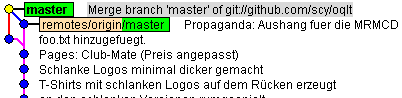
\includegraphics[width=0.8\linewidth]{merge.png}\end{center}
\end{example}
\end{frame}

\subsection{Branches ohne Ende}

\begin{frame}{Branches in Git}
\begin{itemize}
	\item die natürlichste Sache der Welt
	\item ein Branch ist ein Zeiger auf einen kinderlosen Commit\\(eine „Entwicklungsspitze“)
	\item Branches sind (normalerweise) lokal; der Rest der Welt\\sieht deinen Unfug nicht
	\item hin und her mergen zwischen Branches ist trivial
\end{itemize}
\begin{center}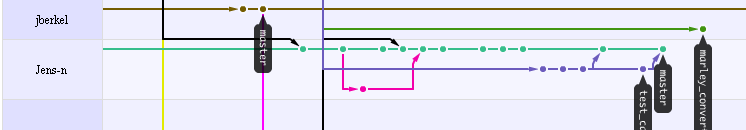
\includegraphics[width=0.8\linewidth]{branches.png}\end{center}
\end{frame}

\begin{frame}{Vorteile}
\begin{itemize}
	\item keine Angst vor Branches
	\item Branches zwischen einzelnen Developern tauschen
	\item Feature-Branches
	\item komplett unterschiedliche Inhalte in einem Repository (Code, Doku, Website, Git-basierter Bugtracker, \ldots)
\end{itemize}
\end{frame}

\section{Die geile Scheiße}

\subsection{Tricks beim Committen}

\begin{frame}{Committen einzelner Änderungen}
\begin{itemize}
	\item Vorteil des Index: Man kann auch nur „halbe“ Dateien committen
	\item \TYPE|git add -p| (für „patch“) erlaubt, einzelne Diff-Hunks für einen Commit auszuwählen
	\item \textbf{Demo!}
\end{itemize}
\end{frame}



\end{document}
